\section{Defining security of QKD}
\label{sec:qkd}

The first Quantum Key Distribution (QKD) protocols were proposed
independently by \textcite{BB84} \--- inspired by early work on
quantum money by \textcite{Wie83} \--- and by \textcite{Eke91}. The
original papers discussed security in the presence of an eavesdropper
that could perform only limited operations on the quantum channel. The
models of security evolved over time \--- a review of these is given
in \secref{sec:qkd.other} \--- and the security criterion used today
was introduced in 2005~\cite{RK05,BHLMO05,Ren05}, the so\-/called
\emph{trace distance criterion}. It was argued that $\rho_{KE}$, the
joint state of the final key $K$ and quantum information gathered by
an eavesdropper $E$, must be close to an ideal key, $\tau_K$, that is
perfectly uniform and independent from the adversary's information
$\rho_E$:
\begin{equation} \label{eq:d} (1-\pabort) D \left(     \rho_{KE},\tau_K \otimes \rho_E \right) \leq \eps \   ,
\end{equation} 
where $\pabort$ is the probability that the protocol
aborts,\footnote{In \textcite{Ren05}, \eqnref{eq:d} was introduced
  with a subnormalized state $\rho_{KE}$, with
  $\trace{\rho_{KE}}=1-\pabort$, instead of explicitly writing the
  factor $(1-\pabort)$. The two formulations are however
  mathematically equivalent.} $D(\cdot,\cdot)$ is the trace
distance\footnote{This metric corresponds to the distinguishing
  advantage between two quantum states, and is formally defined in
  \appendixref{app:op}.} and $\eps \in [0,1]$ is a (small) real
number. This security criterion was discussed within the cryptography
frameworks introduced in \secref{sec:ac} by \textcite{BHLMO05,MR09}
\--- see also \appendixref{app:op}.

We note that \eqnref{eq:d} only captures how much an adversary knows
about the key (called \emph{secrecy} in the QKD literature). A QKD
scheme must additionally guarantee that Alice and Bob hold the same
key with high probability (called \emph{correctness}) and that under
reasonable noisy conditions a QKD scheme produces a key with high
probability (called \emph{robustness}). In this section, we describe
how these security notions fit into the general framework described in
\secref{sec:ac}. For this we first explain in
\secref{sec:qkd.overview} how to use the AC framework to model the
task achieved by a QKD protocol \--- namely constructing a secret key
resource from an insecure quantum channel and an authentic classical
channel \--- and write out the corresponding security
definitions. Then in \secref{sec:security} we show how to derive
secrecy, correctness and robustness from these security
definitions. And finally, in \secref{sec:qkd.other} we review other
security definitions that have appeared in the literature, and explain
how they relate to the trace distance criterion, namely \eqnref{eq:d}.


\subsection{The real and ideal QKD systems}
\label{sec:qkd.overview}

In order to apply the general AC security definition to QKD, we first need to specify the ideal key resource, which we do in \secref{sec:qkd.ideal}. Likewise, we specify in \secref{sec:qkd.protocol} the real QKD system consisting of the protocol, an authentic classical channel and an insecure quantum channel. Plugging these systems in \defref{def:security}, we obtain in \secref{sec:qkd.security} the security criteria for QKD.


\subsubsection{Ideal key}
\label{sec:qkd.ideal}

The goal of a key distribution protocol is to generate a secret key shared between two players, Alice and Bob. One can represent such a resource by a box, one end of which is in Alice's lab, and another in Bob's. It provides each of them with a secret key of a given length, but does not give Eve any information about the key. This is illustrated in \figref{fig:qkd.resource.simple}, and is the key resource we used in the OTP construction [\figref{fig:otp.real}].


\begin{figure}[tb]
  \centering

  \subfloat[Simple ideal key][\label{fig:qkd.resource.simple}A
  resource that always gives a key $k$ to Alice and Bob, and nothing
  to Eve.]{
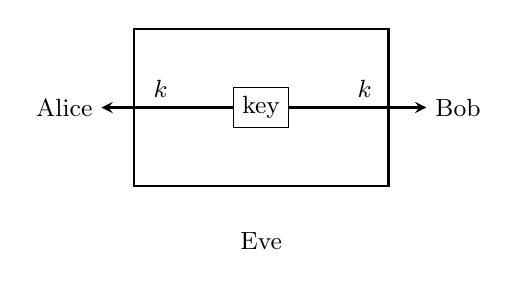
\begin{tikzpicture}[
sArrow/.style={->,>=stealth,thick},
largeResource/.style={draw,thick,minimum width=1.618*2cm,minimum height=2cm}]

\small

\def\u{0} %2/1.618-1

\node[largeResource] (keyBox) at (0,0) {};
\node (alice) at (-2.5,\u) {Alice};
\node (bob) at (2.5,\u) {Bob};
\node (eve) at (0,-1.7) {Eve};
\node[draw] (key) at (0,0) {key};

\draw[sArrow] (key) to node[pos=.55,auto,swap] {$k$} (alice);
\draw[sArrow] (key) to node[pos=.55,auto] {$k$} (bob);

\end{tikzpicture}
} 

\vspace{6pt}

\subfloat[Ideal key with switch][\label{fig:qkd.resource.switch}A
resource that allows Eve to decide if Alice and Bob get a key $k$ or
an error $\bot$.]{
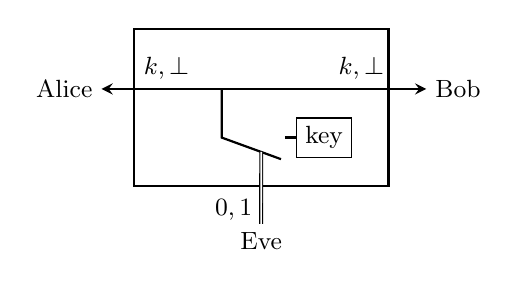
\begin{tikzpicture}[
sArrow/.style={->,>=stealth,thick},
largeResource/.style={draw,thick,minimum width=1.618*2cm,minimum height=2cm}]

\small

\def\u{.236} %2/1.618-1

\node[largeResource] (keyBox) at (0,0) {};
\node (alice) at (-2.5,\u) {Alice};
\node (bob) at (2.5,\u) {Bob};
\node (eve) at (0,-1.7) {Eve};
\node[draw] (key) at (.8,\u/2-.5) {key};
\node (junc) at (-.5,0 |- key.center) {};

\draw[sArrow,<->] (alice) to node[pos=.2,auto] {$k,\bot$} node[pos=.8,auto] {$k,\bot$} (bob);
\draw[thick] (junc.center |- 0,\u) to (junc.center) to node[pos=.666] (handle) {} +(160:-.8);
\draw[thick] (.3,0 |- junc.center) to (key);
\draw[double] (eve) to node[pos=.2,auto] {$0,1$} (handle.center);

\end{tikzpicture}
}

\vspace{6pt}

\subfloat[Probabilistic Ideal
key][\label{fig:qkd.resource.probabilistic}A resource that generates a
perfect key with probability $1-\delta$ and outputs an error $\bot$
with probability $\delta$.]{

% \begin{tikzpicture}[
% sArrow/.style={->,>=stealth,thick},
% thinResource/.style={draw,thick,minimum width=1.618*2cm,minimum height=1cm},
% innersnode/.style={minimum width=.4cm,minimum height=.3cm}]

% \small

% \def\t{2.368} % 1.618+.75
% \def\u{-1.85} % .5+.5+1.7/2
% \def\w{-3.2} % .5+.5+1.7+.5
% \def\v{.118} % 1/1.618-.5
% \def\s{.91}

% \node[thinResource] (keyBox) at (0,0) {};
% \node[draw] (key) at (0,\v/2-.25) {key};
% \node (junc) at (-1.4,0 |- key.center) {};
% \node[yshift=-1.5,above right] at (keyBox.north west) {\footnotesize
%   Secret key $\aK$};
% \node (alice) at (-\t,\v) {};
% \node (bob) at (\t,\v) {};

% \draw[sArrow,<->] (alice.center) to node[pos=.08,auto] {$k,\bot$} node[pos=.92,auto] {$k,\bot$} (bob.center);
% \draw[thick] (junc.center |- 0,\v) to (junc.center) to node[pos=.472] (handle) {} +(160:-.8);
% \draw[thick] (-.6,0 |- junc.center) to (key);

% \node[thinResource] (sim) at (0,\u+.35) {};
% \node[xshift=1.5,below left] at (sim.north west) {\footnotesize
%   $\lozenge_E$};
% \node[innersnode] (a1) at (handle |- 0,\u+.35) {};

% \draw[double] (a1) to node[pos=.55,auto,swap] {$0,1$} (handle.center);

% \end{tikzpicture}
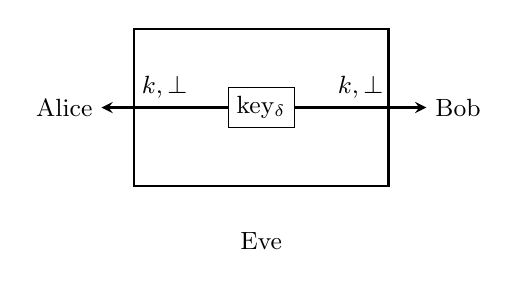
\begin{tikzpicture}[
sArrow/.style={->,>=stealth,thick},
largeResource/.style={draw,thick,minimum width=1.618*2cm,minimum height=2cm}]

\small

\def\u{0} %2/1.618-1

\node[largeResource] (keyBox) at (0,0) {};
\node (alice) at (-2.5,\u) {Alice};
\node (bob) at (2.5,\u) {Bob};
\node (eve) at (0,-1.7) {Eve};
\node[draw] (key) at (0,0) {key$_\delta$};

\draw[sArrow] (key) to node[pos=.5,auto,swap] {$k,\bot$} (alice);
\draw[sArrow] (key) to node[pos=.5,auto] {$k,\bot$} (bob);

\end{tikzpicture}
}

\caption[Secret key resources]{\label{fig:qkd.resource}Some depictions
  of shared secret key resources.}
\end{figure}

However, if we wish to realize such a functionality with QKD, there is
a caveat: an eavesdropper can always prevent any real QKD protocol
from generating a key by cutting or jumbling the communication lines
between Alice and Bob, and this must be taken into account by the
definition of the ideal resource. This box thus also has an interface
accessible to Eve, which provides her with a switch that, when
pressed, prevents the box from generating this key. We depict this in
\figref{fig:qkd.resource.switch}.

If an OTP protocol uses the key generated by the resource of
\figref{fig:qkd.resource.switch}, we need to consider two cases. If
Eve prevents a key from being generated, the construction is trivially
secure \--- in this case, Alice and Bob do not have a key and
therefore cannot send any message. And in the case where a key
is generated, we have the situation depicted by
\figref{fig:qkd.resource.simple}, which is the situation we already
analyzed in \secref{sec:ac.otp}.

As explained above, an adversary can prevent a key from getting
distributed by disrupting the communication channels. But even if no
adversary is present, one might still wish to take into account that,
due to noise or other disturbance, it can happen that no key is
generated. One may in this case be able to bound the probability of
successfully distributing a key, and so the ideal resource constructed
is stronger than that of \figref{fig:qkd.resource.switch} (where there
is no bound on the probability of getting a key), but weaker than that
of \figref{fig:qkd.resource.simple} (where a key is generated with
probability $1$). This middle point is depicted in
\figref{fig:qkd.resource.probabilistic} (where a key is generated
with probability $1-\delta$) and is treated in
\secref{sec:security.rob}.

% If no adversary is present, a filter covers Eve's interface of the
% resource, making it inaccessible to the distinguisher. This filter
% emulates the honest behavior that one expects in the case of a
% non\-/malicious noisy channel. For a protocol and noisy channel that
% together produce a key with probability $1-\delta$, the filter should
% flip the switch on the $E$\=/interface of the ideal key with
% probability $\delta$. This is illustrated in
% \figref{fig:qkd.resource.filter}, and discussed in more detail in
% \secref{sec:security.rob}.

\subsubsection{Real QKD system}
\label{sec:qkd.protocol}

\paragraph{Protocol.}
There exist various types of QKD protocols, which differ by their use of resources and hence practical feasibility \cite{SBCDLP09}. For example, in \emph{entanglement\-/based} protocols, first proposed in \textcite{Eke91}, Alice and Bob use a source of entanglement together with a classical authentic (but otherwise insecure) communication channel to generate their keys. Here, we focus on prepare-and-measure schemes, where instead of having access to entanglement, it is assumed that Alice can send quantum states to Bob. These protocols, for which  \textcite{BB84} is the most prominent example, are technologically less challenging than entanglement-based ones, for they do not require the generation of entanglement. Alice merely has to prepare states and send them to Bob, and Bob has to measure them. 

QKD protocols can roughly be divided into three phases: quantum state
distribution, error estimation and classical post\-/processing. In the
first, Alice sends some quantum states to Bob, who measures them upon
reception, obtaining a classical string, called the \emph{raw key}.
In the error estimation phase, they sample some bits at random
positions in the raw key and estimate the noise on the quantum channel
by comparing these values to what Bob should have obtained. If the
noise level is above a certain threshold, they abort the protocol and
output an error message. If the noise is low enough, they move on to
the third phase, in which they perform error correction and privacy
amplification on their respective strings. Error correction allows Bob
to correct the bits where his raw key is different from
Alice's. Privacy amplification turns the raw key, about which an
adversary may still have partial information, into the final secret
key, i.e., uniform strings $k_A$ and $k_B$ for Alice and Bob,
respectively (which should ideally be equal).

\paragraph{Resources.} 
The security of a QKD protocol depends of course also on the resources
we start with. As mentioned previously, we are interested in making
 statements about two cases. In the presence of an active adversary, we
wish to guarantee that any key generated is secure (soundness). But
this is not sufficient, since a protocol that always aborts and never
distributes a key satisfies such a criterion, but is completely
pointless. We thus also want to guarantee that if no adversary is
present \--- only natural (low) noise \--- a key will be generated
with high probability (completeness).

These two cases are modeled by considering different resources in the
real world. In the case of an active adversary, the resources
available for a prepare\-/and\-/measure scheme are a one-way insecure
quantum channel from Alice to Bob (i.e., Eve may change and insert
messages on the channel) and a classical two-way authentic channel
(i.e., it allows authenticated communication from Alice to Bob and Bob
to Alice, but Eve may also listen in). These are illustrated in
\figref{fig:qkd.real.adv}. Recall that this construction is then
supposed to realize the ideal system depicted in
\figref{fig:qkd.resource.switch}.


\begin{figure}[tb]
  \centering \subfloat[With adversary][\label{fig:qkd.real.adv}Eve's
  interfaces of the channel resources give her full access to the
  quantum communication and allow her to read the messages on the
  authentic channel.]{
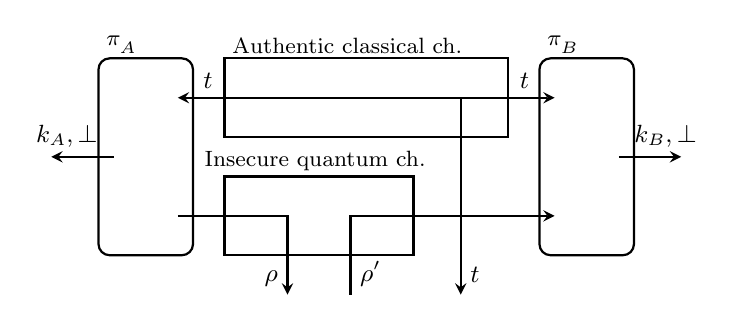
\begin{tikzpicture}[
sArrow/.style={->,>=stealth,thick},
thinResource/.style={draw,thick,minimum width=2.4cm,minimum height=1cm},
longResource/.style={draw,thick,minimum width=3.6cm,minimum height=1cm},
protocol/.style={draw,rounded corners,thick,minimum width=1.2cm,minimum height=2.5cm},
pnode/.style={minimum width=.8cm,minimum height=.5cm}]

\small

\def\t{4} %.6+1.2+.4+1.2*3/2
\def\u{2.8} %1.2/2+.4+1.2*3/2
\def\v{.75}
\def\w{.6} %1.2/2

\node[pnode] (a1) at (-\u,\v) {};
\node[pnode] (a2) at (-\u,0) {};
\node[pnode] (a3) at (-\u,-\v) {};
\node[protocol] (a) at (-\u,0) {};
\node[yshift=-2,above right] at (a.north west) {\footnotesize
  $\pi^{\qkd}_A$};
\node (alice) at (-\t,0) {};

\node[pnode] (b1) at (\u,\v) {};
\node[pnode] (b2) at (\u,0) {};
\node[pnode] (b3) at (\u,-\v) {};
\node[protocol] (b) at (\u,0) {};
\node[yshift=-2,above right] at (b.north west) {\footnotesize $\pi^{\qkd}_B$};
\node (bob) at (\t,0) {};

\node[longResource] (cch) at (0,\v) {};
\node[yshift=-2,above right] at (cch.north west) {\footnotesize
  Authentic classical ch.~$\aA$};
\node[thinResource] (qch) at (-\w,-\v) {};
\node[yshift=-1.5,above] at (qch.north) {\footnotesize
  Insecure quantum ch.~$\aQ$};
\node (eveq1) at (-\w-.4,-1.75) {};
\node (junc1) at (eveq1 |- a3) {};
\node (eveq2) at (-\w+.4,-1.75) {};
\node (junc2) at (eveq2 |- a3) {};
\node (evec) at (\w+\w,-1.75) {};
\node (junc3) at (evec |- b1) {};

\draw[sArrow,<->] (a1) to node[auto,pos=.08] {$t$} node[auto,pos=.92] {$t$}  (b1);
\draw[sArrow] (junc3.center) to node[auto,pos=.9] {$t$} (evec.center);

\draw[sArrow] (a2) to node[auto,pos=.75,swap] {$k_{A},\bot$} (alice.center);
\draw[sArrow] (b2) to node[auto,pos=.75] {$k_{B},\bot$} (bob.center);

\draw[sArrow] (a3) to (junc1.center) to node[pos=.8,auto,swap] {$\rho$} (eveq1.center);
\draw[sArrow] (eveq2.center) to node[pos=.264,auto,swap] {$\rho'$} (junc2.center) to (b3);

\end{tikzpicture}
}

\vspace{6pt}

\subfloat[Without adversary][\label{fig:qkd.real.noise}In a model with
  natural noise, the resources $\aQ$ and $\aA$ are replaced with
  (non\-/malicious) variants $\aQ'$ and $\aA'$ that have
  a blank interface for Eve and a fixed noise model for the channel
  $\aQ'$.]{
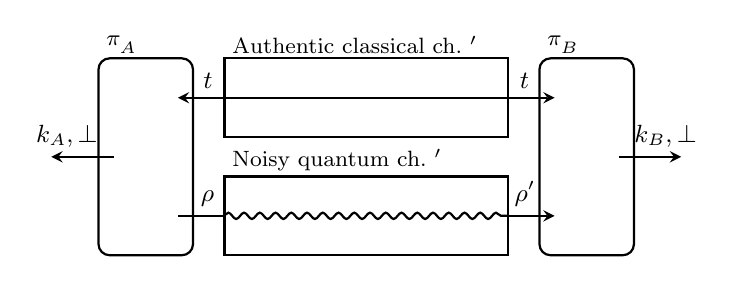
\begin{tikzpicture}[
sArrow/.style={->,>=stealth,thick},
sLine/.style={-,thick},
nLine/.style={-,thick,decorate,decoration={snake,amplitude=.4mm,segment length=2mm,post length=1mm}},
thinResource/.style={draw,thick,minimum width=2.4cm,minimum height=1cm},
longResource/.style={draw,thick,minimum width=3.6cm,minimum height=1cm},
filter/.style={draw,thick,minimum width=1.618cm,minimum height=1cm},
lineFilter/.style={draw,ultra thick,minimum width=.8cm,inner sep=0},
protocol/.style={draw,rounded corners,thick,minimum width=1.2cm,minimum height=2.5cm},
pnode/.style={minimum width=.8cm,minimum height=.5cm}]

\small

\def\t{4} %.6+1.2+.4+1.2*3/2
\def\u{2.8} %1.2/2+.4+1.2*3/2
\def\v{.75}
\def\w{.6} %1.2/2

\node[pnode] (a1) at (-\u,\v) {};
\node[pnode] (a2) at (-\u,0) {};
\node[pnode] (a3) at (-\u,-\v) {};
\node[protocol] (a) at (-\u,0) {};
\node[yshift=-2,above right] at (a.north west) {\footnotesize
  $\pi^{\qkd}_A$};
\node (alice) at (-\t,0) {};

\node[pnode] (b1) at (\u,\v) {};
\node[pnode] (b2) at (\u,0) {};
\node[pnode] (b3) at (\u,-\v) {};
\node[protocol] (b) at (\u,0) {};
\node[yshift=-2,above right] at (b.north west) {\footnotesize $\pi^{\qkd}_B$};
\node (bob) at (\t,0) {};

\node[longResource] (cch) at (0,\v) {};
\node[yshift=-2,above right] at (cch.north west) {\footnotesize
  Authentic classical ch.~$\aA'$};
\node[longResource] (qch) at (0,-\v) {};
\node[yshift=-1.5,above right] at (qch.north west) {\footnotesize
  Noisy quantum ch.~$\aQ'$};

% \node[filter] (qchf) at (-\w,-3*\v) {};
% \node[xshift=2,below left] at (qchf.north west) {\footnotesize $\sharp_E$};
% \node[lineFilter] (cchf) at (2*\w,-3*\v) {};
% \node[right] at (cchf.east) {\footnotesize $\flat_E$};

% \node[xshift=-.6cm] (qchl) at (qch.center) {};
% \node[xshift=.6cm] (qchr) at (qch.center) {};
% \node (qchl) at (qchfl |- qchf.north) {};
% \node (qchr) at (qchfr |- qchf.north) {};
% \node (junc1) at (qchfl |- a3) {};
% \node (junc2) at (qchfr |- a3) {};

% \node (junc3) at (cchf.center |- b1) {};

\draw[sArrow,<->] (a1) to node[auto,pos=.08] {$t$} node[auto,pos=.92] {$t$}  (b1);
% \draw[sArrow] (junc3.center) to node[auto,pos=.9] {$t$} (cchf);

\draw[sArrow] (a2) to node[auto,pos=.75,swap] {$k_{A},\bot$} (alice.center);
\draw[sArrow] (b2) to node[auto,pos=.75] {$k_{B},\bot$} (bob.center);

\draw[sLine] (a3) to node[pos=.65,auto] {$\rho$} (qch.west);
\draw[nLine] (qch.west) to (qch.east);
\draw[sArrow] (qch.east) to node[pos=.35,auto] {$\rho'$} (b3);

% \draw[sArrow] (qchl.center) to (qchfl.center) to (qchfr.center) to (qchr.center);

\end{tikzpicture}
}

\caption[QKD system]{\label{fig:qkd.real}The real QKD system \---
  Alice has access to the left interface, Bob to the right interface
  and Eve to the lower interface \--- consists of the protocol
  $(\pi^{\qkd}_A,\pi^{\qkd}_B)$, the insecure quantum channel $\aQ$ in
  \subref{fig:qkd.real.adv} [and a noisy channel $\aQ'$ in
  \subref{fig:qkd.real.noise}] and two-way authentic classical channel
  $\aA$ (or $\aA'$, respectively). As before, arrows represent the
  transmission of (classical or quantum) messages.

  The protocols of Alice and Bob $(\pi^{\qkd}_A,\pi^{\qkd}_B)$ abort
  if they detect too much interference, i.e., if $\rho'$ is not
  similar enough to $\rho$ to obtain a secret key of the desired
  length. They run the classical post\-/processing over the authentic
  channel, obtaining keys $k_A$ and $k_B$. The message $t$ depicted on
  the two-way authentic channel represents the entire transcript of
  the classical communication between Alice and Bob during the
  protocol.}
\end{figure}

The quantum channel is used in the protocol when Alice sends the
qubits she prepared to Bob. This channel may be completely under the
control of Eve, who could apply any operation allowed by physics to
what is sent over the channel. The authentic channel is used during
the next two phases of the protocol, in which Alice and Bob estimate
the noise in their raw keys and perform the post-processing. Such a
channel faithfully transmits messages between Alice and Bob, but
provides Eve with a copy as well.  Since an authentic channel can be
constructed from an insecure channel and a short shared secret key,
QKD is sometimes referred to as a \emph{key expansion}
protocol.\footnote{We model QKD this way in \secref{sec:smt}.}

The second case is modeled by resources which are not controlled by
Eve anymore. Instead, the quantum channel has a fixed noise model and
the authentic channel does not provide copies of the messages to
Eve. This is drawn in \figref{fig:qkd.real.noise}. With these assumed
resources, the ideal resource one wishes to construct is given by
\figref{fig:qkd.resource.probabilistic}.


\subsubsection{Security}
\label{sec:qkd.security}

For the following, we denote by $(\pi^\qkd_A,\pi^\qkd_B)$ the QKD
protocol, with $\pi^\qkd_A$ and $\pi^\qkd_B$ the converters applied by
Alice and Bob, respectively.  We furthermore denote by $\aQ$ the
insecure quantum channel and by $\aA$ the authentic classical channel,
as drawn in \figref{fig:qkd.real.adv}. Their non\-/malicious
counterparts are denoted $\aQ'$ and $\aA'$,
respectively, as in \figref{fig:qkd.real.noise}. Finally,
let $\aK$ be the secret key resource of
\figref{fig:qkd.resource.switch}, and $\aK'$ the secret key
resource of \figref{fig:qkd.resource.probabilistic}. Applying
\defref{def:security}, we find that $(\pi_A^{\qkd},\pi_B^{\qkd})$
constructs $\aK$ from $\aQ$ and $\aA$ within
$\eps$ if 
\begin{equation} \label{eq:qkd.security}
  \exists \sigma_E, \quad \pi_A^{\qkd}\pi_B^{\qkd}(\aQ \| \aA)
  \close{\eps} \aK \sigma_E,
\end{equation}
and  $(\pi_A^{\qkd},\pi_B^{\qkd})$
constructs $\aK'$ from $\aQ'$ and $\aA'$ within
$\eps'$ if 
\begin{equation} \label{eq:qkd.robust}
  \pi_A^{\qkd}\pi_B^{\qkd}(\aQ'
  \| \aA') \close{\eps'} \aK'.
\end{equation}
Note that no simulator is needed in \eqnref{eq:qkd.robust}, because
both the real and ideal system have a blank interface for Eve.  The
left- and right-hand sides of \eqnref{eq:qkd.security} are illustrated
in Figs.~\ref{fig:qkd.real.adv} and \ref{fig:qkd.resource.sim}, and
the left- and right-hand sides of \eqnref{eq:qkd.robust} are
illustrated in Figs.~\ref{fig:qkd.real.noise} and
\ref{fig:qkd.resource.probabilistic}. These two conditions are
decomposed into simpler criteria in \secref{sec:security}.


\begin{figure}[tb]
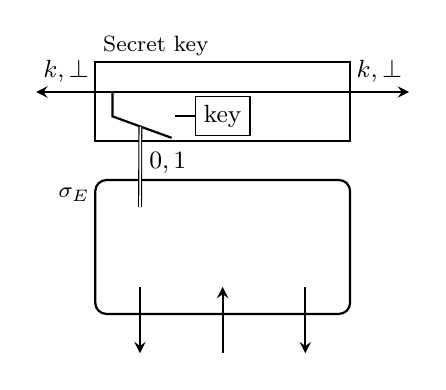
\begin{tikzpicture}[
sArrow/.style={->,>=stealth,thick},
thinResource/.style={draw,thick,minimum width=1.618*2cm,minimum height=1cm},
simulator/.style={draw,rounded corners,thick,minimum width=1.618*2cm,minimum height=1.7cm},
snode/.style={minimum width=1.1cm,minimum height=1.2cm},
innersnode/.style={minimum width=.4cm,minimum height=.3cm}]

\small

\def\t{2.368} % 1.618+.75
\def\u{-1.85} % .5+.5+1.7/2
\def\w{-3.2} % .5+.5+1.7+.5
\def\v{.118} % 1/1.618-.5
\def\s{1.05}

\node[thinResource] (keyBox) at (0,0) {};
\node[draw] (key) at (0,\v/2-.25) {key};
\node (junc) at (-1.4,0 |- key.center) {};
\node[yshift=-1.5,above right] at (keyBox.north west) {\footnotesize
  Secret key $\aK$};
\node (alice) at (-\t,\v) {};
\node (bob) at (\t,\v) {};

\draw[sArrow,<->] (alice.center) to node[pos=.08,auto] {$k,\bot$} node[pos=.92,auto] {$k,\bot$} (bob.center);
\draw[thick] (junc.center |- 0,\v) to (junc.center) to node[pos=.472] (handle) {} +(160:-.8);
\draw[thick] (-.6,0 |- junc.center) to (key);

\node[simulator] (sim) at (0,\u) {};
\node[xshift=1.5,below left] at (sim.north west) {\footnotesize
  $\sigma_E$};
\node[innersnode] (a1) at (-\s,\u+.35) {};
\node[innersnode] (a2) at (-\s,\u-.35) {};
\node[innersnode] (b2) at (\s,\u-.35) {};
\node[innersnode] (c2) at (0,\u-.35) {};

\node (evel) at (-\s,\w) {};
\node (evec) at (0,\w) {};
\node (ever) at (\s,\w) {};

\draw[double] (a1) to node[pos=.55,auto,swap] {$0,1$} (handle.center);
\draw[sArrow] (a2) to (evel.center);
\draw[sArrow] (evec.center) to (c2);
\draw[sArrow] (b2) to (ever.center);

\end{tikzpicture}

\caption[Ideal key \& simulator]{\label{fig:qkd.resource.sim}The key resource from
\figref{fig:qkd.resource.switch} with a simulator $\sigma_E$. This
corresponds to the ideal world in \eqnref{eq:qkd.security}.}
\end{figure}

\subsection{Reduction to the trace distance criterion}
\label{sec:security}

By applying the general AC security definition to QKD, we obtained two
criteria, \eqnsref{eq:qkd.security} and \eqref{eq:qkd.robust},
capturing soundness and completeness, respectively. In this section we
derive the trace distance criterion, \eqnref{eq:d}, introduced at the
beginning of \secref{sec:qkd}, from \eqnref{eq:qkd.security}. We first
show in \secref{sec:security.dist} that the distinguishing advantage
used in the previous sections reduces to the trace distance between
the quantum states gathered by the distinguisher interacting with the
real and ideal systems. Then in \secref{sec:security.simulator}, we
determine the simulator $\sigma_E$ of the ideal system. In
\secref{sec:security.simple} we decompose the resulting security
criterion into a combination of \emph{secrecy} \--- the trace distance
criterion \--- and \emph{correctness} \--- the probability that
Alice's and Bob's keys differ. In the last section,
\ref{sec:security.rob}, we consider the security condition of
\eqnref{eq:qkd.robust}, which captures (security) guarantees in the
absence of a malicious adversary.  We show how this condition can be
used to model the \emph{robustness} of the protocol, i.e., the
probability that the protocol aborts with non\-/malicious noise.

\subsubsection{Trace distance}
\label{sec:security.dist}

The security criteria given in \eqnsref{eq:qkd.security} and
\eqref{eq:qkd.robust} are defined in terms of the distinguishing
advantage between resources. To simplify these equations, we rewrite
them in terms of the trace distance between the states held by the
distinguisher at the end of the protocol in the real and ideal
settings. \textcite{Hel76} proved that the advantage a distinguisher
has in guessing whether it was provided with one of two states with
equal priors, $\rho$ or $\sigma$, is given by the trace distance
between the two, $D(\rho,\sigma)$.\footnote{Actually, \textcite{Hel76}
  solved a more general problem, in which the states $\rho$ and
  $\sigma$ are picked with a priori probabilities $p$ and $1-p$,
  respectively, instead of $1/2$ as in the definition of the
  distinguishing advantage.} A proof of this along with a discussion
of different operational interpretations of the trace distance is
given in \appendixref{app:op}.

We start with the criterion given by~\eqnref{eq:qkd.robust}. The two resources on the left- and right-hand sides of \eqnref{eq:qkd.robust} simply output classical strings (a key or error message) at Alice and Bob's interfaces. Let these pairs of strings be given by the joint probability distributions $P_{AB}$ and $\tilde{P}_{AB}$. The distinguishing advantage between the two resources is thus simply the distinguishing advantage between these probability distributions \--- a distinguisher is given a pair of strings sampled according to either $P_{AB}$ or $\tilde{P}_{AB}$ and has to guess from which distribution it was sampled \--- i.e., 
\[ 
  d\left( \pi_A^{\qkd}\pi_B^{\qkd}(\aQ' \| \aA'), \aK' \right) = d(P_{AB},\tilde{P}_{AB}).
   \] 
 As stated above, the distinguishing advantage between two quantum states is equal to their trace distance, and in the special case where the states are classical \--- i.e., given by two probability distributions \--- the trace distance between the classical states is equal to the total variational distance between the corresponding probability distributions. Thus $d(P_{AB},\tilde{P}_{AB})= D(P_{AB},\tilde{P}_{AB})$, where we use the same notation for both the trace distance and total variational distance, since the latter is a special case of the former. Putting the two together we get
\[ 
d\left( \pi_A^{\qkd}\pi_B^{\qkd}(\aQ' \| \aA')
  , \aK' \right) = D(P_{AB},\tilde{P}_{AB}),
 \] 
  where $P_{AB}$ and $\tilde{P}_{AB}$ are the distributions of the strings output by the real and ideal systems, respectively.

  The resources on the left- and right-hand sides of
  \eqnref{eq:qkd.security} are slightly more complex than those in
  \eqnsref{eq:qkd.robust}. They first output a state $\varphi_C$ at
  the $E$\=/interface, namely the quantum states that Alice sends over
  the insecure quantum channel. Without loss of generality, the
  distinguisher now applies any map $\cE : \lo{C} \to \lo{CE'}$
  allowed by quantum physics to this state, obtaining
  $\rho_{CE'} = \cE(\varphi_C)$ and puts the $C$ register back on the
  insecure channel for Bob, keeping the part in $E'$. Finally, the
  systems output some keys (or error messages) at the $A$ and
  $B$\=/interfaces, and all classical messages exchanged during the
  error estimation and post\-/processing at the $E$\=/interface \---
  this captures the fact that the classical communication is
  public.\footnote{We sometimes refer to the entire sequence of these
    messages as the \emph{classical transcript} of the protocol.} This
  sequence of interactions of the distinguisher with the real or ideal
  QKD systems is illustrated in \figref{fig:qkd.distinguisher}.

  \begin{figure}[tb]
    \centering
    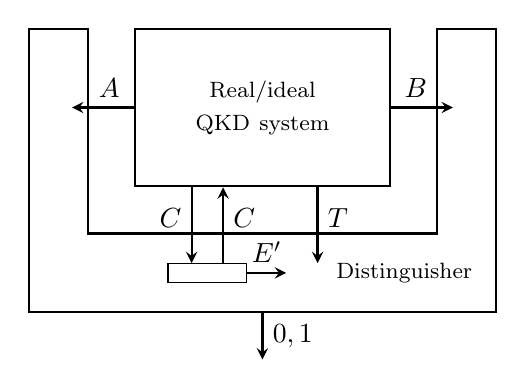
\begin{tikzpicture}[
      sArrow/.style={->,>=stealth,thick},
      largeResource/.style={draw,thick,minimum width=1.618*2cm,minimum
        height=2cm}]

      \node[largeResource,text width=3cm,text centered] (R) at (0,0) {\footnotesize Real/ideal QKD system};

      \draw[thick] (-1.618-1.35,1) -- ++(.75,0) -- ++(0,-2.6)  --
++(1.618*2+1.2,0)  -- ++(0,2.6) -- ++(.75,0) -- ++(0,-3.6) --
++(-1.618*2-2.7,0) -- cycle;

     \node[draw,minimum width=1cm] (E) at (-.7,-2.1) {$\cE$};
     \node at (1.8,-2.1) {\footnotesize Distinguisher};
     
     \draw[sArrow] (R) to node[auto,swap,pos=.4] {$A$} (-1.618-.8,0);
     \draw[sArrow] (R) to node[auto,pos=.4] {$B$} (1.618+.8,0);
     \draw[sArrow] (-.9,0 |- R.south) to node[auto,swap,pos=.4] {$C$}
     (-.9,0 |- E.north);
     \draw[sArrow] (-.5,0 |- E.north) to node[auto,swap,pos=.6] {$C$}
     (-.5,0 |- R.south);
     \draw[sArrow] (.7,0 |- R.south) to node[auto,pos=.4] {$T$}
     (.7,0 |- E.north);
    \draw[sArrow] (E.east |- 0,-2.1) to node[auto] {$E'$}
     (.3,-2.1);

     \draw[sArrow] (0,-2.6) to node[auto] {$0,1$} (0,-3.2);
    \end{tikzpicture}
    \caption[Distinguisher for QKD]{\label{fig:qkd.distinguisher}The
      distinguisher interacting with either the real or ideal QKD
      system first receives a register $C$ containing the quantum
      states sent from Alice to Bob. It applies a map
      $\cE : \lo{C} \to \lo{CE'}$ of its choice, keeps the $E'$
      register and puts $C$ back in the insecure channel. Finally, it
      gets the transcript of the classical communication $T$, and
      Alice's and Bob's outputs $A$ and $B$. It thus holds a state
      $\rho_{ABE'T}$, which it measures to decide if it was
      interacting with the real or ideal system.}
  \end{figure}
  

  Let $\rho^{\cE}_{ABE}$ be the tripartite state held by a
  distinguisher interacting with the real system, and
  $\tilde{\rho}^{\cE}_{ABE}$ the state held after interacting with the
  ideal system, where the registers $A$ and $B$ contain the final keys
  or error messages, and the register $E$ holds both the state
  $\rho_{E'}$ obtained from tampering with the quantum channel and the
  classical transcript. Distinguishing between these two systems thus
  reduces to maximizing over the distinguisher strategies (the choice
  of $\cE$) and distinguishing between the resulting states,
  $\rho^{\cE}_{ABE}$ and $\tilde{\rho}^{\cE}_{ABE}$:
\[ 
d\left( \pi_A^{\qkd}\pi_B^{\qkd}(\aQ \| \aA) , \aK \sigma_E \right)
= \max_{\cE} d\left( \rho^{\cE}_{ABE},\tilde{\rho}^{\cE}_{ABE} \right).
 \]
 Using again the equality between trace distance and distinguishing
 advantage, we obtain that the advantage a distinguisher has in
 guessing whether it holds the state $\rho^{\cE}_{ABE}$ or
 $\tilde{\rho}^{\cE}_{ABE}$ is given by the trace distance between
 these states, i.e.,
\[ 
  d\left( \pi_A^{\qkd}\pi_B^{\qkd}(\aQ \| \aA) , \aK \sigma_E \right)
= \max_{\cE} D\left(\rho^{\cE}_{ABE},\tilde{\rho}^{\cE}_{ABE} \right). 
\]

The distinguishing advantage between the real and ideal systems of
\eqnref{eq:qkd.security} thus reduces to the trace distance between
the quantum states gathered by the distinguisher. In the following, we
usually omit ${\cE}$ where it is clear that we are maximizing over the
distinguisher strategies, and simply express the security criterion
as \begin{equation} \label{eq:qkd.security.1}
  D(\rho_{ABE},\tilde{\rho}_{ABE}) \leq \eps, \end{equation} where
$\rho_{ABE}$ and $\tilde{\rho}_{ABE}$ are the quantum states gathered
by the distinguisher interacting with the real and ideal systems,
respectively.


\subsubsection{Simulator}
\label{sec:security.simulator}

In the real setting [\figref{fig:qkd.real.adv}], Eve has full control
over the quantum channel and obtains the entire classical transcript
of the protocol. So for the real and ideal settings to be
indistinguishable, a simulator $\sigma^{\qkd}_E$ must generate the
same communication as in the real setting. This can be done by
internally running Alice's and Bob's protocol
$(\pi^{\qkd}_A,\pi^{\qkd}_B)$, producing the same messages at Eve's
interface as the real system. However, instead of letting this
(simulated) protocol decide the value of the key as in the real
setting, the simulator ignores these values and only checks whether a
key is actually produced or whether an error message is generated
instead. It then operates the switch on the secret key resource
accordingly. We illustrate this in \figref{fig:qkd.ideal}.

% The simulator, which is plugged into the $E$\=/interface of the ideal key
% resource (as depicted in \figref{fig:qkd.resource.sim}), can decide
% if the key is generated, but does not obtain any information about
% the value of the key. 

\begin{figure}[tb]


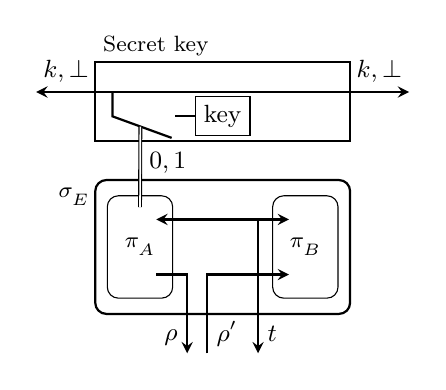
\begin{tikzpicture}[
sArrow/.style={->,>=stealth,thick},
thinResource/.style={draw,thick,minimum width=1.618*2cm,minimum height=1cm},
simulator/.style={draw,rounded corners,thick,minimum width=1.618*2cm,minimum height=1.7cm},
innersim/.style={minimum width=.83cm,minimum height=1.3cm},
innersnode/.style={minimum width=.4cm,minimum height=.3cm}]

\small

\def\t{2.368} % 1.618+.75
\def\u{-1.85} % .5+.5+1.7/2
\def\w{-3.2} % .5+.5+1.7+.5
\def\v{.118} % 1/1.618-.5
\def\s{1.05}

\node[thinResource] (keyBox) at (0,0) {};
\node[draw] (key) at (0,\v/2-.25) {key};
\node (junc) at (-1.4,0 |- key.center) {};
\node[yshift=-1.5,above right] at (keyBox.north west) {\footnotesize
  Secret key $\aK$};
\node (alice) at (-\t,\v) {};
\node (bob) at (\t,\v) {};

\draw[sArrow,<->] (alice.center) to node[pos=.08,auto] {$k,\bot$} node[pos=.92,auto] {$k,\bot$} (bob.center);
\draw[thick] (junc.center |- 0,\v) to (junc.center) to node[pos=.472] (handle) {} +(160:-.8);
\draw[thick] (-.6,0 |- junc.center) to (key);

\node[simulator] (sim) at (0,\u) {};
\node[xshift=1.5,below left] at (sim.north west) {\footnotesize
  $\sigma^{\qkd}_E$};
\node[innersim,rounded corners,draw] (pleft) at (-\s,\u) {\footnotesize $\pi^{\qkd}_A$};
\node[innersim,rounded corners,draw] (pright) at (\s,\u) {\footnotesize $\pi^{\qkd}_B$};
\node[innersnode] (a1) at (-\s,\u+.35) {};
\node[innersnode] (a2) at (-\s,\u-.35) {};
\node[innersnode] (b1) at (\s,\u+.35) {};
\node[innersnode] (b2) at (\s,\u-.35) {};

\node (evel) at (-.45,\w) {};
\node (juncl) at (evel |- a2) {};
\node (evec) at (-.2,\w) {};
\node (juncc) at (evec |- a2) {};
\node (ever) at (.45,\w) {};
\node (juncr) at (ever |- a1) {};

\draw[double] (a1) to node[pos=.55,auto,swap] {$0,1$} (handle.center);
\draw[sArrow,<->] (a1) to (b1);
\draw[sArrow] (juncr.center) to node[pos=.852,auto] {$t$} (ever.center);
\draw[sArrow] (a2) to (juncl.center) to node[pos=.805,auto,swap] {$\rho$} (evel.center);
\draw[sArrow] (evec.center) to node[pos=.25,auto,swap] {$\rho'$} (juncc.center) to (b2);

\end{tikzpicture}


\caption[Simulator for QKD]{\label{fig:qkd.ideal}The ideal QKD system \--- Alice  has access to the left interface, Bob to the right interface and Eve   to the lower interface \--- consists of the ideal secret key   resource and a simulator $\sigma^{\qkd}_E$.}
\end{figure}

The security criterion from \eqnref{eq:qkd.security.1} can now be simplified by noting that with this simulator, the states of the ideal and real systems are identical when no key is produced. The outputs at Alice's and Bob's interfaces are classical elements of the set $\{\bot\} \cup \cK$, where $\bot$ symbolizes an error and $\cK$ is the set of possible keys. The states of the real and ideal systems can be written as
\begin{align*}  \rho_{ABE} & = p^\bot \proj{\bot_A,\bot_B} \otimes
  \rho^\bot_E \\
  & \qquad + \sum_{k_A,k_B \in \cK} p_{k_A,k_B} \proj{k_A,k_B} \otimes
  \rho^{k_A,k_B}_E,\\
  \tilde{\rho}_{ABE} & = p^\bot \proj{\bot_A,\bot_B}
  \otimes \rho^\bot_E \\ & \qquad +\frac{1}{|\cK|} \sum_{k \in \cK} \proj{k,k}
  \otimes \sum_{k_A,k_B \in \cK} p_{k_A,k_B} \rho^{k_A,k_B}_E,
\end{align*}
where $p_{k_A,k_B}$ is the probability of Alice getting the key $k_A$
and Bob getting $k_B$, and $p^\bot$ is the probability of an abort.
Plugging this in \eqnref{eq:qkd.security.1} we get
\begin{equation} \label{eq:qkd.security.2} D\left(
    \rho_{ABE},\tilde{\rho}_{ABE}\right) = (1- p^{\bot})
  D\left(\rho^{\top}_{ABE},\tau_{AB} \otimes \rho^{\top}_{E}\right)
  \leq \eps, 
  \end{equation}
where
 \begin{equation} \label{eq:qkd.security.tmp} \rho^{\top}_{ABE}
  \coloneqq \frac{1}{1- p^{\bot}} \sum_{k_A,k_B \in \cK} p_{k_A,k_B}
  \proj{k_A,k_B} \otimes \rho^{k_A,k_B}_E 
\end{equation}
is the renormalized state of the system conditioned on not aborting
and $\tau_{AB} \coloneqq \frac{1}{|\cK|} \sum_{k \in \cK} \proj{k,k}$
is a perfectly uniform shared key. As previously, the $E$ register
contains the quantum side information that Eve collects about the
states being sent as well as the entire classical transcript of the
error estimation and post\-/processing.

\subsubsection{Correctness \& secrecy}
\label{sec:security.simple}

We now break \eqnref{eq:qkd.security.2} up into two components, often referred to as \emph{correctness} and \emph{secrecy}, and recover the security definition for QKD introduced in \textcite{RK05,BHLMO05,Ren05}. The correctness of a QKD protocol refers to the probability that Alice and Bob end up holding different keys. We say that a protocol is \emph{$\eps_{\corr}$\=/correct} if for all adversarial strategies,
\begin{equation}
  \label{eq:qkd.cor}
  \Pr \left[ K_A \neq K_B \right] \leq \eps_{\corr},
\end{equation}
where $K_A$ and $K_B$ are random variables over the alphabet $\cK \cup \{\bot\}$ describing Alice's and Bob's outputs.\footnote{This can  equivalently be written as $(1-p^\bot)\Pr \left[ K^\top_A \neq     K^\top_B \right] \leq \eps_{\corr}$, where $p^\bot$ is the   probability of aborting and $K^\top_A$ and $K^\top_B$ are Alice and   Bob's keys conditioned on not aborting.} The secrecy of a QKD protocol measures how close the final key is to a distribution that is uniform and independent of the adversary's system. Let $p^\bot$ be the probability that the protocol aborts, and $\rho^\top_{AE}$ be the resulting state of the $AE$ subsystems conditioned on not aborting. A protocol is \emph{$\eps_{\secr}$\=/secret} if for all adversarial strategies,
\begin{equation}
  \label{eq:qkd.sec}
  (1-p^\bot) D\left(\rho^\top_{AE},\tau_A \otimes \rho^{\top}_E\right)
  \leq \eps_{\secr},
\end{equation}
where the distance $D(\cdot,\cdot)$ is the trace distance and $\tau_A$
is the fully mixed state.\footnote{\eqnref{eq:qkd.sec} was already
  introduced at the beginning of \secref{sec:qkd} as \eqnref{eq:d}.}

\begin{thm}
  \label{thm:qkd}
  If a QKD protocol is $\eps_{\corr}$\=/correct and
  $\eps_{\secr}$\=/secret, then \eqnref{eq:qkd.security} is satisfied
  for $\eps = \eps_{\corr} + \eps_{\secr}$.
\end{thm}

This theorem can be proven by using the triangle inequality of the
trace distance to bound \eqnref{eq:qkd.security.2} in terms of the sum
of correctness and secrecy. For completeness, a proof is given in
\appendixref{app:proofs}. This result may also be found in
\textcite{BHLMO05}.

The converse statement can also be shown: if \eqnref{eq:qkd.security} holds for some $\eps$, then the corresponding QKD protocol is both $\eps$\=/correct and $2\eps$\=/secret.\footnote{The factor $2$ is due to the existence quantifier over simulators $\sigma_E$ in the security definition. We cannot exclude that for some specific QKD protocol there exists a  simulator $\bar{\sigma}^\qkd_E$, different from the one used in this proof, that generates a   state $\bar{\rho}_E$ satisfying   $D\left(\rho^{\top}_{AE},\tau_{A} \otimes \bar{\rho}^{\top}_E\right)   \leq D\left(\rho^{\top}_{AE},\tau_{A} \otimes \rho^{\top}_E\right)$.   However, by the triangle inequality we also have that for any   $\bar{\rho}_E$,   $D\left(\rho^{\top}_{AE},\tau_{A} \otimes \bar{\rho}^{\top}_E\right)  \geq \frac{1}{2} D\left(\rho^{\top}_{AE},\tau_{A} \otimes     \rho^{\top}_E\right)$.  Hence the failure $\eps$ of the generic simulator used in this proof   cannot be more than twice as large compared to the optimal one.}


\subsubsection{Robustness}
\label{sec:security.rob}

Correctness and secrecy, as described above, capture the soundness of QKD in the presence of a
malicious Eve, as specified by
\eqnref{eq:qkd.security}.  This is however not sufficient: a QKD protocol which
always aborts without producing any key trivially satisfies
\eqnref{eq:qkd.security} with $\eps=0$, but is obviously not a useful
protocol at all! This is where the second condition, namely
\eqnref{eq:qkd.robust}, is relevant. The real system must not only be
indistinguishable from ideal when an adversary is present and
manipulating the channel, but also when one has a simple noisy
channel, with a blank adversarial interface. In this case, we expect a
secret key to be generated successfully with high probability. This is
captured by considering the strong ideal key resource $\aK'$ from
\figref{fig:qkd.resource.probabilistic} which produces a key with
probability $1-\delta$. If the real system does not generate a key
with the same probability, this immediately results in a gap
noticeable by the distinguisher.

The probability that the real protocol generates a key depends on the
noise introduced by the noisy channel $\aQ'$ [illustrated in
\figref{fig:qkd.real.noise}]. Suppose that this noise is parametrized
by a value $q$, e.g., a depolarizing channel with probability $q$. For
every $q$, the protocol has a probability of aborting, $\delta$, which
is called the \emph{robustness}. Let $\aQ_q$ denote a channel with
this noise model, and let $\aK_\delta$ denote the key resource which
produces an error with a fixed probability
$\delta$. \eqnref{eq:qkd.robust} can thus be phrased as
\begin{equation} \label{eq:robustness} \pi_A^{\qkd}\pi_B^{\qkd}(\aQ_q \|
  \aA') \close{\eps} \aK_\delta
  ,\end{equation} 
  where varying $q$ and $\delta$ results in a family of real and ideal systems.

One can then show that the failure $\eps$ from \eqnref{eq:robustness} is bounded by $\eps_{\corr}+\eps_{\secr}$. Note that this statement is only useful if the probability of aborting, $\delta$, is small for reasonable noise models $q$.

\begin{lem} \label{lem:robustness}
If the resources from \eqnref{eq:robustness} are parametrized such that $\aK_\delta$ aborts with exactly the same probability as the protocol $(\pi_A^{\qkd},\pi_B^{\qkd})$ run on the noisy channel $\aQ_q$, then the completeness of the protocol is bounded by the soundness, i.e.,  
\begin{equation*} d\left( \pi_A^{\qkd}\pi_B^{\qkd}(\aQ_q \| \aA')
  ,\aK_\delta\right)  \leq d\left(
  \pi_A^{\qkd}\pi_B^{\qkd}(\aQ \| \aA),\aK \sigma^{\qkd}_E\right),
\end{equation*} 
where the simulator $\sigma^{\qkd}_E$ is the one used in the previous sections, introduced in \secref{sec:security.simulator}, \figref{fig:qkd.ideal}.
\end{lem}

A proof of this is provided in \appendixref{app:proofs}.


\subsection{Other security criteria}
\label{sec:qkd.other}


\subsubsection{Accessible information}
\label{sec:qkd.other.ai}

As mentioned at the beginning of this section, the trace distance
criterion was only introduced in
2005~\cite{RK05,BHLMO05,Ren05}. Earlier works, e.g.,
\textcite{May96,BBBMR00,SP00}, used a notion of security directly
inspired from classical cryptography, where key techniques such as
\emph{advantage distillation}, \emph{error correction} and
\emph{privacy amplification} were developed
\cite{BBR88,Mau93,AC93,BBCM95}. More concretely, if one denotes an
$n$-bit key random variable by $K$ and the adversary's classical side
information by $Z$, in these works a key was considered secure if the
mutual information per bit between the two is small, i.e.,
$\frac{1}{n}\Ii(K;Z) \leq \eps$, where $\Ii(K;Z) = \Hh(K) -
\Hh(K|Z)$. It was later realized \cite{Mau94,MW00} that the mutual
information per bit is not appropriate in the asymptotic setting,
since $\eps(n) \to 0$ does not imply that the total information about
the key is also small, i.e., one may still have
$n\eps(n) \nrightarrow 0$. It was therefore considered preferable to
directly bound the total information about the key,
$\Ii(K;Z) \leq \eps$.

In the case of QKD, the side information may be quantum, and the
joint system of the key and side information is given by a state
$\rho_{KE}$. The \emph{accessible information} between $K$ and $E$ is
obtained by measuring the $E$ system, and taking the mutual
information between $K$ and the measurement outcome, i.e., 
\begin{equation} \label{eq:localqkd} \Ii_{\text{acc}} (K;E)_\rho
  \coloneqq \max_{\{\Gamma_z\}_z} \Ii(K;\Gamma_Z(E)) \leq \eps,
 \end{equation} 
 where $\Gamma_Z(E)$ is the random variable resulting from measuring
 the $E$ system with the POVM $\{\Gamma_z\}_z$ and as before,
 $\Ii(K;Z) = \Hh(K) - \Hh(K|Z)$ is the mutual information.

 Since measuring a quantum system can only diminish the information it
 provides, one always has $\Ss(K|E) \leq \Hh(K|Z)$ for any random
 variable $Z$ obtained by measuring the $E$ system of a bipartite
 state $\rho_{KE}$, where $\Ss(\cdot)$ is the von Neumann
 entropy. Using the continuity of the conditional von Neumann
 entropy~\cite{AF04}, this can by bounded by its trace distance from
 uniform, namely\footnote{See \corref{cor:AF04} in
   \appendixref{app:op} for a proof of this.}
 \[
 n - \Ss(K|E) \leq 8 \delta n + 2h(2\delta),
 \] 
 where $\delta$ is the trace distance between $\rho_{KE}$ and
 $\tau_K \otimes \rho_E$ and $h(p) = - p \log p - (1-p) \log (1-p)$ is
 the binary entropy. The trace distance criterion thus provides a
 bound on the accessible information.

 Crucially, however, the converse does not hold. As shown in
 \textcite{KRBM07}, it is possible to find a joint state $\rho_{K E}$
 of an $n$-bit key $K$ and the adversary's information~$E$ that
 satisfies \eqnref{eq:localqkd} with $\eps = 2^{-0.18n}$, but knowledge
 of the first $n-1$ bits $K_1$ of $K=K_1K_2$ allow the last bit $K_2$
 to be guessed perfectly.\footnote{This phenomenon is known as
   \emph{information locking} and further examples may be found in
   \textcite{DHLST04,Win17}.} More precisely, if one knows $K_1$ there
 is a way to measure the quantum system $E$ such that the outcome,
 $\Gamma_{Z'}(K_1E)$ is a perfect guess for
 $K_2$,\footnote{\textcite{BHLMO05} show that if $\eps < 2^{-n}$ then
   information locking cannot be exploited, and the adversary's
   advantage in guessing $K_2$ remains exponentially small.} i.e.,
 \[\Ii(K_2;\Gamma_{Z'}(K_1E)) = 1.\]

 To see why this is problematic, suppose that the two parts of the
 key, $K_1$ and $K_2$, are used for One-Time Pad encryption (cf.\
 \secref{sec:ac.otp}) of two messages $M_1$ and $M_2$, respectively,
 of which the first is already known to an eavesdropper (e.g., because
 it contains some publicly available information).  Given $M_1$, the
 eavesdropper can, by listening to the ciphertext, infer $K_1$. This,
 in turn, allows her to apply the measurement yielding $Z'$ to $E$,
 which provides information about $K_2$, and hence also about $M_2$.

 The example emphasises the relevance of \emph{composability}, i.e.,
 the principle that any reasonable notion of \emph{security} should
 have the property that if two cryptographic schemes are considered
 secure then this should also be the case for their
 combination. Criterion~\eqref{eq:localqkd} does not satisfy this
 principle. If a key $K$ generated by a QKD protocol satisfies
 \eqnref{eq:localqkd} then, by definition, it is guaranteed that an
 adversary cannot infer $K$.  But the composition of this QKD protocol
 with the One-Time Pad encryption, which by itself is a perfectly
 secure protocol, is insecure. This is clearly problematic, for such
 compositions of protocols are ubiquitous in cryptography.

 To see how the real\-/world ideal\-/world paradigm avoids this issue,
 imagine a protocol that generates a key consisting of two parts,
 $K_1$ and $K_2$, with the (undesirable) properties as in the example
 from \textcite{KRBM07} described above. The distinguisher could then
 use~$K_1$ to measure~$E$ and check whether the outcome~$Z'$
 determines~$K_2$.  If this is the case then the distinguisher knows
 that it was interacting with the real system ($B=0$), otherwise it
 must have been the ideal one ($B=1$). The distinguisher could thus
 correctly guess the bit~$B$, i.e., the protocol would not meet the
 criterion of being indistinguishable from an ideal system. Hence,
 although the key generation protocol may still satisfy earlier
 criteria such as \eqnref{eq:localqkd}, it would be considered
 insecure, as it should be.

 It is interesting nonetheless to understand what construction a
 security definition like the accessible information corresponds
 to. We discuss this in \secref{sec:alternative.memoryless}, where we
 show that if one assumes that the adversary has no quantum memory,
 then the accessible information is a sufficient security criterion.
 
\subsubsection{Adversarial models}
\label{sec:qkd.other.models}

The definition of cryptographic security introduced in \secref{sec:ac}, \defref{def:security}, does not explicitly mention an adversary. The notion of an adversary is embedded in the distinguisher, which is used to measure the distance between real and ideal systems. The distinguishing metric thus has a dual role: performing the most powerful attack possible and measuring whether this attack was successful \--- i.e., whether it allows real and ideal systems to be distinguished. The reduction to the trace distance criterion discussed in \secref{sec:security} separates these two notions. The trace distance criterion itself, \eqnref{eq:d}, can be seen as the measure of whether the attack resulting in the adversary holding the system $E$ is successful. For this condition to make sense as a security definition, one has to consider all possible adversarial behaviors, i.e., take the maximum of \eqnref{eq:d} over all possible states $\rho_{KE}$ that may occur.

Historically, these two aspects \--- the attack and the criterion for
measuring whether the attack is successful \--- were treated
separately. Early security proofs for QKD, e.g., \textcite{BBBSS92},
did not consider the most powerful attack an eavesdropper could
perform, but only \emph{individual attacks}. These are attack
strategies where the adversary performs an identical operation on each
qubit on the quantum channel and keeps only classical information
$Z$. The information held by Alice, Bob, and Eve is then modeled by
independent and identically distributed (i.i.d.) random variables.

\emph{Collective attacks} \--- a generalization of individual attacks
that allows the eavesdropper to keep quantum information, but still
forces her to perform the same operation on every qubit \--- were
proposed in \textcite{BM97b,BBBvdGM02}. In this setting, one has to
use von Neumann entropy instead of Shannon entropy to measure the
adversary's information about the raw key and compute the achievable
rate \cite{DW05}. Although the adversary's interactions with the
quantum channel are restricted to i.i.d.\ operations, this class of
attacks is particularly important, since proof techniques developed
later \cite{Ren05,Ren07,CKR09,DFR20,AFRV19} show how one can reduce the most
general attack strategies to such a limited one.

The first security proof for QKD that considered a fully general adversary \--- performing \emph{coherent} attacks \--- is attributed to \textcite{May96,May01}. It was then followed by other simpler proofs \cite{BBBMR00,BBBMR06,SP00}. 
%These works made minor changes to the accessible information criterion, \eqnref{eq:localqkd}. In \textcite{May96,May01} the author used $n - \Hh(K|Z) \leq \eps$, where $n$ is the length of the final key, since one could imagine an attack strategy that results in a deterministic key with $H(K) = 0$. 
In \textcite{BBBMR00,BBBMR06,SP00} the authors point out that security does not hold conditioned on the protocol terminating with a secret key. Instead, one should prove that the probability of the event that the protocol does not abort  \emph{and} that the adversary has non-trivial information about the key is negligible. However, the works discussed above still use basically classical security definitions, such as those based on the accessible information.
 
\subsubsection{Expressing weaker security criteria within the AC framework}
\label{sec:qkd.other.ac}

As discussed above, the early security definitions implicitly imposed
a restriction on the set of possible attack strategies that an
adversary could pursue. Within the modern real-world ideal-world
paradigm, or, more precisely, the AC framework, one can understand
these restrictions as limitations on the distinguisher that tries to
guess whether it is interacting with the real or ideal system. That
is, one does not consider the full set of possible distinguishers, but
only a restricted subset that, e.g., performs i.i.d.\ operations or
takes its final decision by measuring the $E$ system alone, not the
joint $KE$ system.

Alternatively one may also represent these definitions in the AC
framework either by replacing the resources in the ideal setting by
weaker ones, or the resources available in the real setting by
stronger ones. To illustrate the latter, recall that, within the
description of \secref{sec:qkd.overview}, the insecure quantum channel
used by Alice and Bob allows Eve to perform arbitrary operations on
the quantum messages sent. If instead one would provide the players
with a stronger resource that allows Eve to perform only i.i.d.\
operations or allows her to access classical information only, one
would recover weaker security definitions. This is developed in more
detail in \secref{sec:alternative.memoryless}.

Using such an approach, one may still regard the older security
definitions as ``composable'', provided one is aware of the fact that
the real resources are now weaker. In other words, the weaker
definitions do not guarantee that a secret key is obtained from an
authentic classical channel and a completely insecure quantum channel,
but still ensures that a secret key is obtained from some (less
insecure) quantum channel that limits Eve's tampering.

We note that this approach is applicable much more generally, i.e.,
beyond quantum cryptography.  For example, the notion of security
known as \emph{stand\-/alone}~\cite{Gol04} makes the assumption that
the dishonest party does not interact with the environment during the
execution of the protocol. By introducing a resource that restricts
the distinguisher's behavior accordingly, this security definition can
be shown to actually guarantee security, albeit only in a setting
where honest parties have access to such a resource. Similarly, early
definitions of blindness in delegated quantum computing
\cite[DQC;][]{BFK09,FK17} are not known to construct the expected
ideal resource for DQC \--- one which takes the input from the client,
only leaks a bound on the computation size to the server, and returns
a (possibly wrong) computation result to the client
\cite{DFPR14}. However, they do construct a weaker resource which does
not provide the honest player with the result of the computation. This
example is discussed again in \secref{sec:dqc}. A further example are
results in the bounded storage model by \textcite{Unr11}, who obtains
composable security if one limits the number of times a protocol is
run \--- we discuss these further in \secref{sec:open.other}.

\subsubsection{Asymptotic versus finite-size security}

The trace distance criterion, \eqnref{eq:d}, was introduced in
\textcite{RK05,BHLMO05,Ren05} and the relation to composable security
frameworks has been discussed in \textcite{BHLMO05,MR09} \--- see also
\appendixref{app:op}. Security proofs for QKD with respect to this
criterion were developed at the same time
\cite{CRE04,RGK05,Ren05}. Although these new security proofs arguably
use the right security definition, they only prove security
asymptotically. This means that instead of computing the failure
$\eps$ for specific parameters of the protocol, one shows that
$\eps(n) \to 0$ when $n \to \infty$, where $n$ is a parameter that
quantifies some resource, typically the number of quantum signals sent
during the protocol. This does not allow the failure to be evaluated
for any implementation of the protocol, since implementations must
necessarily generate a key in finite time, and hence with finite
resources.

In the asymptotic setting one often demands that the function
$\eps(n)$ be \emph{negligible}, i.e., smaller than $1/p(n)$ for any
polynomial $p(\cdot)$ \--- for example, $\eps(n)$ could be
exponentially small in $n$. The reasoning is usually that honest
players are polynomially bounded, so they will never run the protocol
more than $p(n)$ times and the accumulated error $p(n)\eps(n)$ is then
still negligible. Although such a requirement is standard in
cryptography, it is not directly useful for practical purposes, as
already indicated above.  For example, a protocol with a failure given
by a function $\eps(n)$ which is exponentially small for $n \geq
10^{10^{10}}$ but equal to $1$ otherwise, where $n$ is the number of
signals exchanged between the players, is asymptotically secure, and
yet completely insecure for any realistic parameters. Conversely, the
function $\eps(n) = 10^{-18}$ is considered insecure in the asymptotic
setting, but it guarantees that the protocol can be run once per
second for the lifetime of the universe, and still have an accumulated
error substantially smaller than $1$.

This illustrates that asymptotic security claims can be highly
ambiguous. It is thus necessary to prove finite security bounds if one
wishes to actually use a cryptographic scheme. This has been done for
basic protocols in, e.g.,
\textcite{ILM07,SR08,STS10,TLGR12,HT12,TL17}. For more advanced
protocols, which are specifically designed to be implementable with
imperfect hardware, finite-size security claims can be found, e.g., in
\textcite{LCWXZ14} for decoy\-/state QKD (which will be discussed in
\secref{sec:attacks:countermeasures}), in~\textcite{YinChen} for
twin-field QKD \cite{Lucamarinietal}, and in \textcite{CXCLTL14} for
measurement\-/device\-/independent QKD (which will be discussed in
\secref{sec:alternative.semi}).

%\begin{rem}[Finite vs.\ negligible failure]

%\end{rem}

\subsubsection{Variations of the trace distance criterion}
\label{sec:qkd.other.variations}

An alternative definition for $\eps$\=/secrecy has been proposed in the literature instead of the trace distance criterion \cite{TSSR10,TLGR12}:
\begin{equation}\label{eq:alternative.sec}
  (1-\pabort)\min_{\sigma_E}D\left(\rho_{KE}, \tau_K \otimes
    \sigma_E\right) \leq \eps.\end{equation}
This alternative notion is equivalent to the standard definition of secrecy [\eqnref{eq:d}] up to a factor $2$, hence any QKD scheme proven secure with one definition is  still secure according to the other, with a minor adjustment of the failure parameter $\eps$. However, we do not know how to derive this alternative notion from a  composable framework. In particular, it is not clear if the failure $\eps$ from \eqnref{eq:alternative.sec} is additive under parallel composition. For example, the concatenation of two keys that each, individually, satisfy \eqnref{eq:alternative.sec}, could possibly have distance from uniform greater than $2\eps$.\footnote{The arXiv version of \textcite{TLGR12} was updated to use \eqnref{eq:d} instead.}


%%% Local Variables:
%%% TeX-master: "main.tex"
%%% End:
